% This is samplepaper.tex, a sample chapter demonstrating the
% LLNCS macro package for Springer Computer Science proceedings;
% Version 2.20 of 2017/10/04
%
\documentclass{article}
%\documentclass[runningheads]{llncs}
%
\usepackage{graphicx}
\usepackage[subrefformat=parens,labelformat=parens]{subcaption}
\usepackage{epsfig}
\usepackage{mathrsfs}
\usepackage{times}
\usepackage{makeidx}
\usepackage{amsmath}
\usepackage{algorithm}
\usepackage{algorithmic}
%\usepackage{subfigure}
%\usepackage{subcaption}
\usepackage{multicol}
\usepackage{array}
\usepackage{siunitx}
\usepackage{balance} % This allows for the even columns in the final page, just insert \balance in the last page, e.g., before the reference list
\usepackage{cite}
%\usepackage{setspace}
\usepackage{etoolbox}
\newtoggle{blindcopy}
%\toggletrue{blindcopy}
\usepackage{hhline}
\usepackage{booktabs}
\usepackage{rotating}
\usepackage{multirow}
\usepackage{wasysym}
\usepackage{xcolor}
\usepackage{adjustbox}
\usepackage{slashbox}
\usepackage{threeparttable}
\usepackage{blindtext}

% Used for displaying a sample figure. If possible, figure files should
% be included in EPS format.
%
% If you use the hyperref package, please uncomment the following line
% to display URLs in blue roman font according to Springer's eBook style:
% \renewcommand\UrlFont{\color{blue}\rmfamily}

\begin{document}
	%
	\title{Extended Abstract for the Thesis:\\Performance Estimation, Testing, and Control of Cyber-Physical Systems Employing Non-Ideal Communications Networks}
	%
	%\titlerunning{Abbreviated paper title}
	% If the paper title is too long for the running head, you can set
	% an abbreviated paper title here
	%
%	\author{Richard Candell\thanks{National Institute of Standards and Technology, United States of America, 100 Bureau Drive, Gaithersburg, MD 20899. \url{http://www.nist.gov}}\\Universit\'e de Bourgogne}
	\author{Richard Candell\\Universit\'e de Bourgogne}

	%
	\maketitle            
	%
	\begin{abstract}
		
			Wireless technology is a key enabler of the promises of Industry 4.0 (Smart Manufacturing). As such, wireless technology will be adopted as a principal mode of communication within the factory beginning with the factory enterprise and eventually being adopted for use within the factory workcell.  Factory workcell communication has particular requirements on latency, reliability, scale, and security that must first be met by the wireless communication technology used.  Wireless is considered a non-ideal form of communication in that when compared to its wired counterparts, it is considered less reliable (lossy) and less secure.  These possible impairments lead to delay and loss of data in industrial automation system where determinism, security, and safety is considered paramount.  This thesis investigates the wireless requirements of the factory workcell and applicability of existing wireless technology, it presents a modeling approach to discovery of architecture and data flows using SysML, it provides a method for the use of graph databases to the organization and analysis of performance data collected from a testbed environment, and finally provides an approach to using machine learning in the evaluation of cyberphysical system performance.\vspace{2mm}
		
%			La technologie sans fil est un catalyseur clé des promesses de l'industrie 4.0 (fabrication intelligente). En tant que telle, la technologie sans fil sera adoptée comme mode de communication principal au sein de l'usine, en commençant par l'entreprise d'usine et finalement adoptée pour une utilisation au sein de la cellule de travail de l'usine. La communication des cellules de travail en usine a des exigences particulières en matière de latence, de fiabilité, d'échelle et de sécurité qui doivent d'abord être satisfaites par la technologie de communication sans fil utilisée. Le sans fil est considéré comme une forme de communication non idéale dans la mesure où, par rapport à ses homologues câblés, il est considéré comme moins fiable (avec perte) et moins sécurisé. Ces dégradations possibles entraînent un retard et une perte de données dans un système d'automatisation industrielle où le déterminisme, la sécurité et la sûreté sont considérés comme primordiaux. Cette thèse étudie les exigences sans fil de la cellule de travail de l'usine et l'applicabilité de la technologie sans fil existante, elle présente une approche de modélisation de la découverte de l'architecture et des flux de données à l'aide de SysML, elle fournit une méthode d'utilisation des bases de données graphiques pour l'organisation et l'analyse des données de performance collectés à partir d'un environnement de banc d'essai, et fournit enfin une approche de l'utilisation de l'apprentissage automatique dans l'évaluation des performances du système cyberphysique.
		
%		\keywords{smart manufacturing, industry 4.0, factory communications, wireless, smart manufacturing, test, measurement, machine learning, databases, sysml, abstract modeling.}
		
	\end{abstract}
	%
	%
	%
	\section{Introduction}
Cyber-physical systems (CPS) are defined as a holistic integration of computing, networking, and physical processes.  Implicit within these systems are feedback connections in which the computing and networking devices affect the physical systems directly.  Traditionally, industrial computation was performed using dedicated electronics with analog process variables and control signals being communicated over twisted-pair wires.  As automation capabilities evolved, serial communications architectures such as the common fieldbus were adopted.  With the advent of the Internet and Cloud Computing, Internet Protocol (IP) was adopted for more advanced data collection and control applications.  In such applications, reliability and latency requirements were not overly difficult to achieve given the existing technologies; however applications requiring tight feedback timing and reliability were not addressed as the protocols primarily targeted slower flow-based processes and building automation.  Discrete manufacturing requirements remained largely unaddressed.  To answer the call of discrete manufacturing requirements, routable industrial IP protocols such as Common Internet Protocol (CIP), SERCOS III, and Profinet by Siemens were developed to guarantee latency, reliability, and interoperability between systems.  However, given that these protocols are often IP-routable and share a common communication medium, these types of systems are limited in their ability to meet the performance demands of the physical systems or guarantee security.   As wired protocols, they can lack flexibility and mobility demanded by modern industrial applications.
Communication strategies that jointly address reliability, timing, scale, and power are needed to meet the needs of future industrial control systems.  Proponents of advanced manufacturing systems such as those defined by Industry 4.0 and the Industrial Internet Consortium state that existing protocols are not capable of meeting all the demands of industry.  The future factory will require untethered situationally-aware communications, heavy reliance on automation to include robotics, and an increased cognitive cybersecurity posture.  It is not certain if feedback control of robot motion is necessary; however future communication systems must address strict latency and data reliability requirements for discrete sensors, actuators, and robot end-effectors while maintaining security.  With the adoption of wireless communications in the factory, existing protocols such as IEEE 802.11 and IEEE 802.15.4 will not be capable of meeting reliability demands, round-trip latencies under 10ms, or scalability to dozens of devices within individual work-cells and hundreds or thousands of devices within an entire factory system.    

Wireless communication is inherently more prone to latency and delay than wired counterparts.  In addition, wireless communication implies the utilization of the electromagnetic spectrum which is a publicly accessible medium with constrained capacity and more prone to cyber-attack.  While transmitted data can by digitally protected through authentication and encryption, wireless devices are prone to interference and jamming by both rogue and friendly emitters exacerbating the reliability and latency concern impacting factory performance without compromising data security.  Wireless communication in factories is often constrained by battery life and most certainly constrained by the availability of the electromagnetic spectrum.   As the reliance on wireless devices within the factory continues, steps toward developing a more robust wireless factory communications network must be developed. These steps include:

\begin{itemize}
	\item[$\star$] The automation system must become situationally aware and adaptive to knowledge of the trends in electromagnetic spectrum occupancy and acute events; and
	
	\item[$\star$] Intelligence of the automation system must move closer to the physical system.  This means moving the intelligence for control to the actuator; and  
	
	\item[$\star$] Performance test methods must be developed and incorporated into the industrial fringe devices.  The test methods must be dependable and at the same time easy to use by factory personal not trained in the technicalities of wireless communication; and
	
	\item[$\star$] Existing Wireless communications protocols must be analyzed and adapted, and new protocols must be developed to balance reliability, latency, and scalability; and
	 
	\item[$\star$] Security of the network must be maintained and must include availability as a paramount characteristic.
\end{itemize}

This thesis includes development of test approaches for measuring the performance of industrial wireless networks deployed within smart manufacturing work-cells.  Thus the primary goal of this thesis is the discovery of methods and approaches to the evaluation of industrial uses cases performance for those use case in which wireless communication technology is used as the principal mode of communication.  The primary motivation of the research is to discover practical test and evaluation methods for assessing performance of an industrial workcell thereby improving security, safety, and reliability in general.   Findings and results of the thesis work are included within the thesis and published as journal articles and conference proceedings.  Resulting data is also made available.

	\section{Contributions and Thesis Organization}
	
		\begin{figure}[!tbhp]
			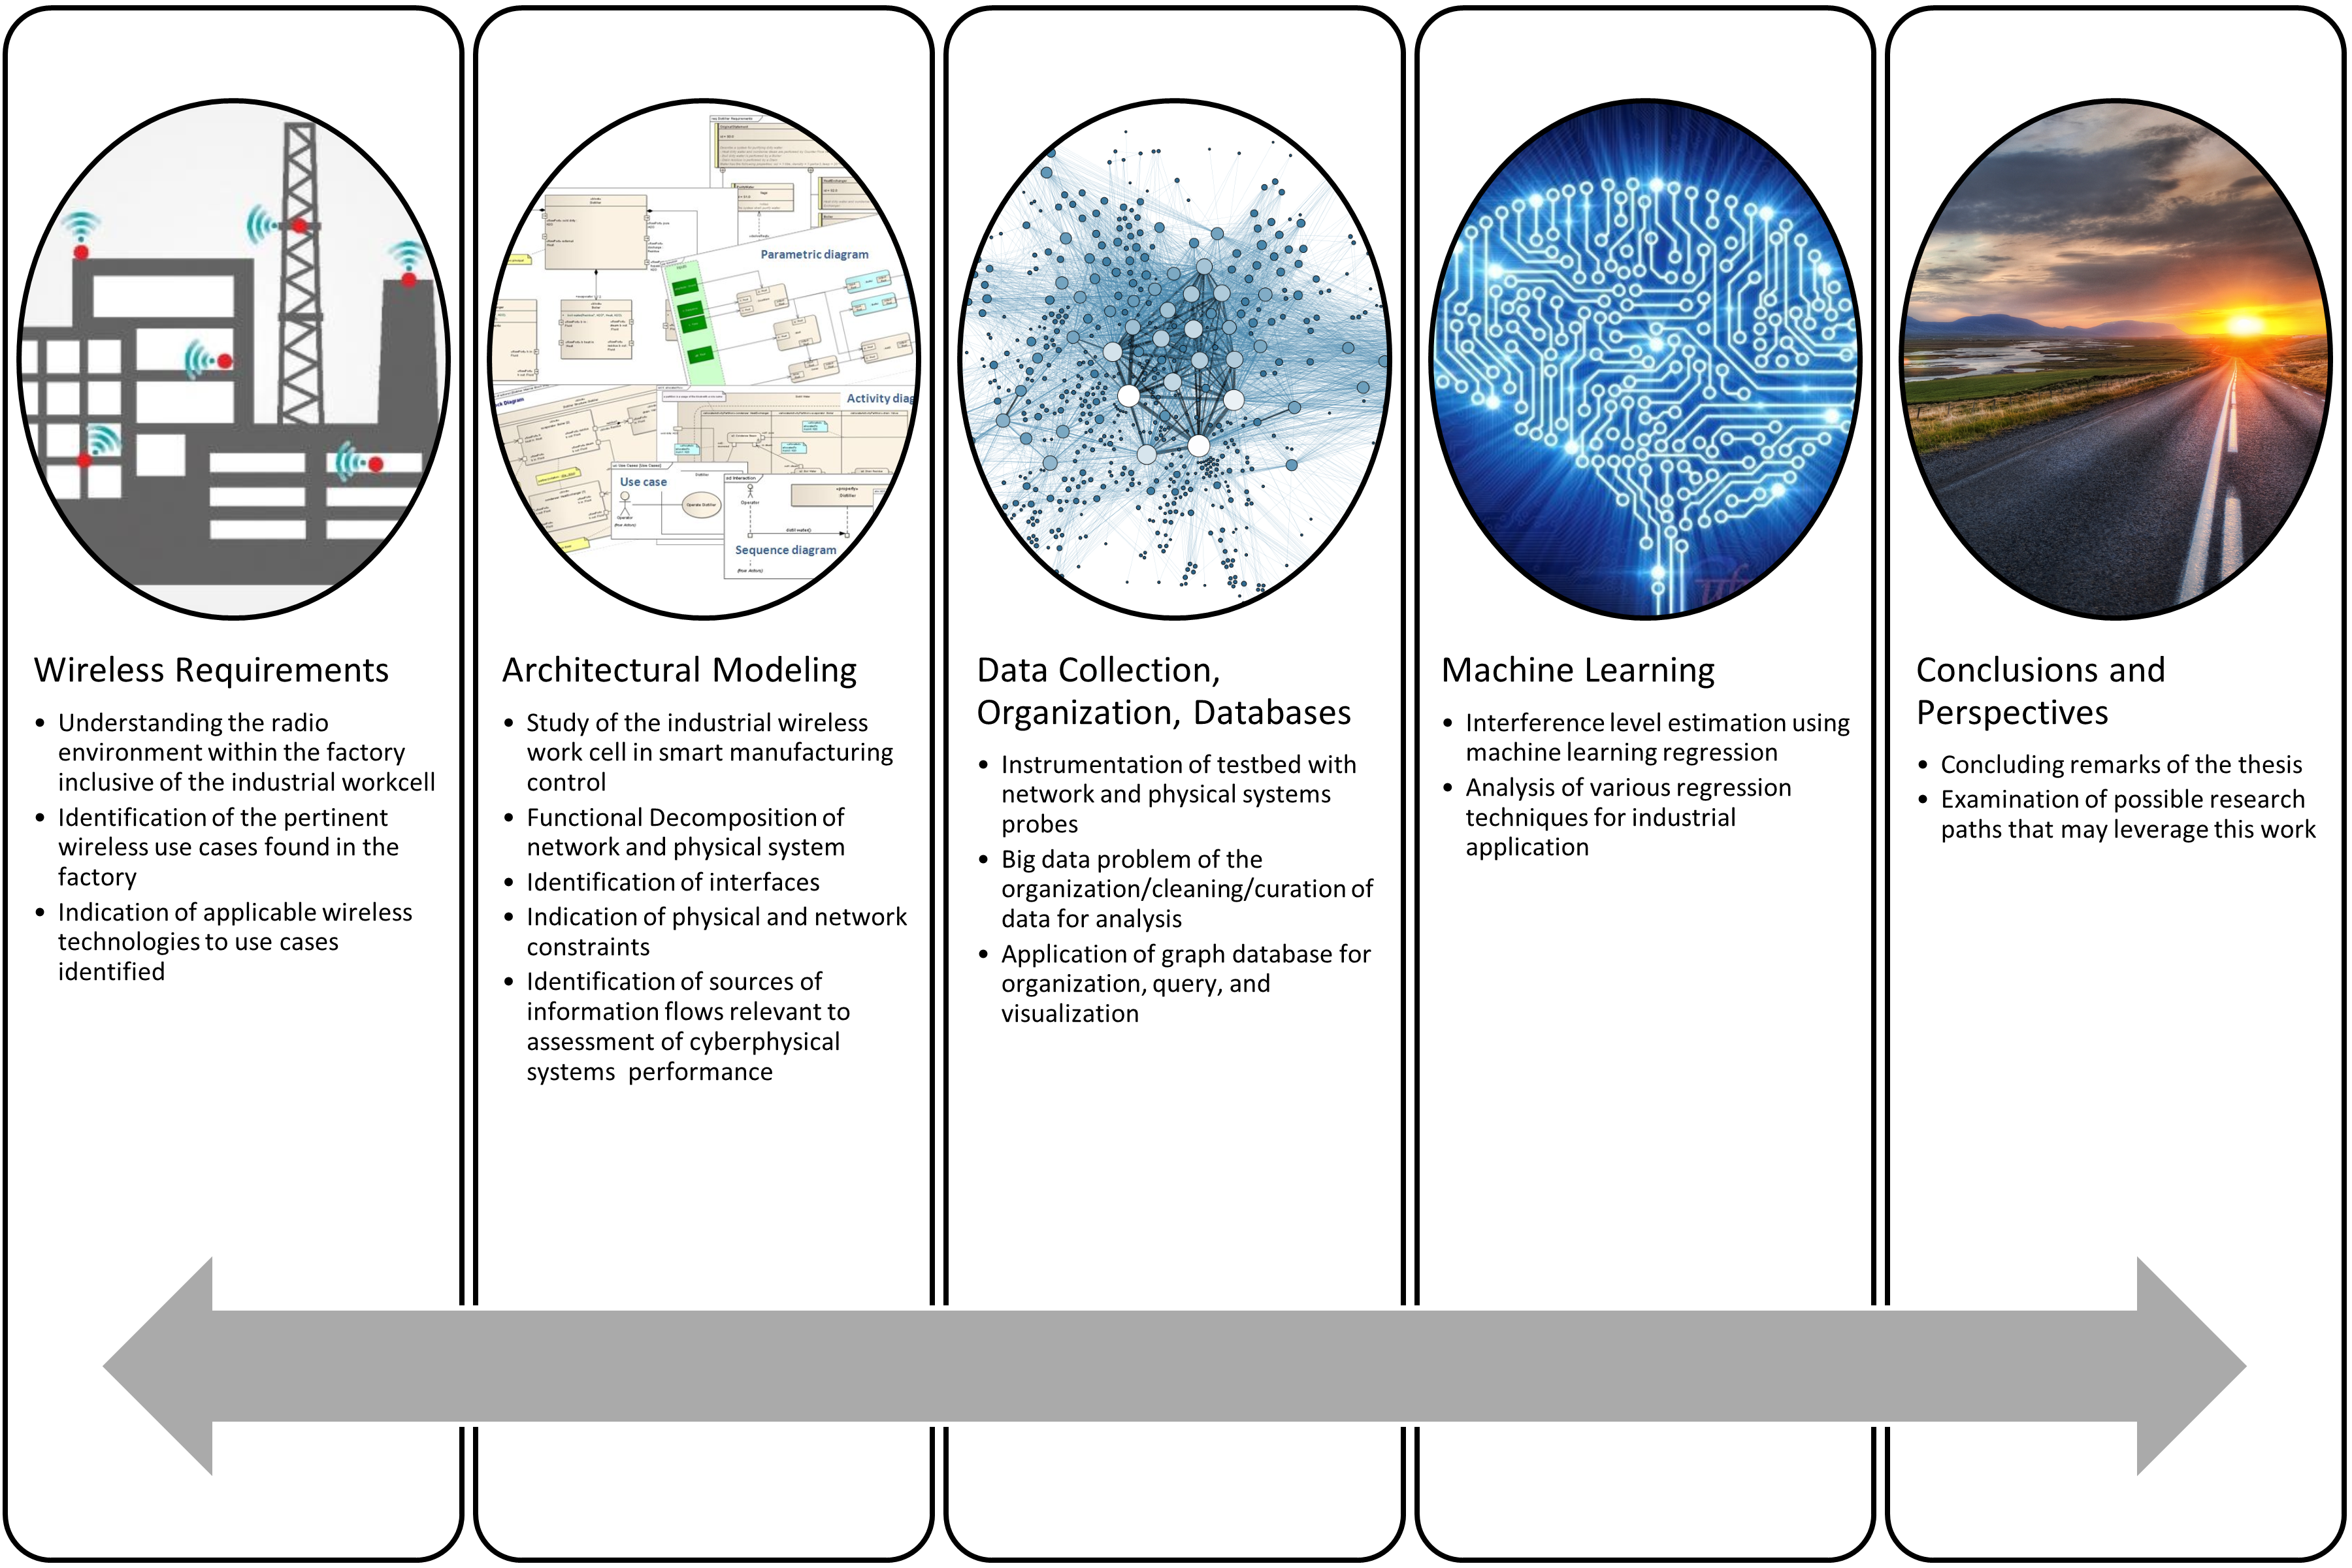
\includegraphics[width=\linewidth]{images/contributions}
			\caption{Contribution areas and organization of this thesis.}
			\label{fig:intro:contr-org}
		\end{figure}
		
		This thesis is presented in three major parts.  In Part I, the thesis provides a historical introduction to the context of smart manufacturing.  It presents the premises of industrial wireless technology, key challenges to using wireless within a factory environment, and the accepted indicators that are currently used in the application of wireless within factory environments. Then, the existing state of the art is presented to orient the reader for the thesis contribution.  This state of the art includes a discussion of the industrial wireless technology landscape, standards, and a tentative mapping of those technologies to application domains.  A discussion of the systems modeling approaches is then provided with a focus on the Systems Markup Language.  Then a discussion of approaches to the use of databases follows   In Part II, \textit{Thesis Contributions}, the technical contributions of this thesis are presented.  Finally, in Part III, the thesis provides a detailed discussion of the four major contributions of this thesis work.  Concluding remarks and future direction are provided as an opinion of the thesis candidate.  
		
		The thesis contributions are presented as follows according to the demonstrated contributions to the state of the art:
		
		\begin{description}
			\item[Requirements] An examination of the wireless technology landscape is conducted.  Existing and future wireless technologies are assessed for their appropriate applicability to industrial use cases.
			
			\item[Modeling] In an effort to better understand the architectural composition of the workcell using industrial wireless communication, modeling techniques are used to identify and decomposed the parts, interfaces, and data flows.  SysML is adopted for this process and a proposed modeling library is created and presented.  The model with conceptual diagram shown in Fig.~\ref{fig:sysmlex} is made publicly available independent of the tool that was used to create the model.
			
			\item[Application of Graph Database] A method (Figures.~\ref{gdbappl:fig:database:work-flow} and~\ref{gdbappl:fig:real-schema}) is developed for collecting, cleaning, organizing, and presenting the cyberphysical performance indicators of experiments run within the NIST Industrial Wireless Testbed. The method developed utilizes the Neo4j graph database and is presented as a novel approach as compared to traditional approaches using relational database, spreadsheets, and raw file processing.
			
			\item[Machine Learning] A machine learning technique is developed and applied to the prediction of signal-to-interference levels within a wireless factory workcell network employing a robot arm within a force-seeking apparatus as shown in Fig.~\ref{fig:photo-forceseeker}  The machine learning method allows a trained network to accurately determine the signal-to-interference level using the physical state of the robot arm rather than the state of the wireless link itself as shown in Fig~\ref{ftml-conf:fig:results-BP}.
		\end{description}
	
		%
		% REQS FIGURE
		%
		\begin{figure}[t]
			\centering
			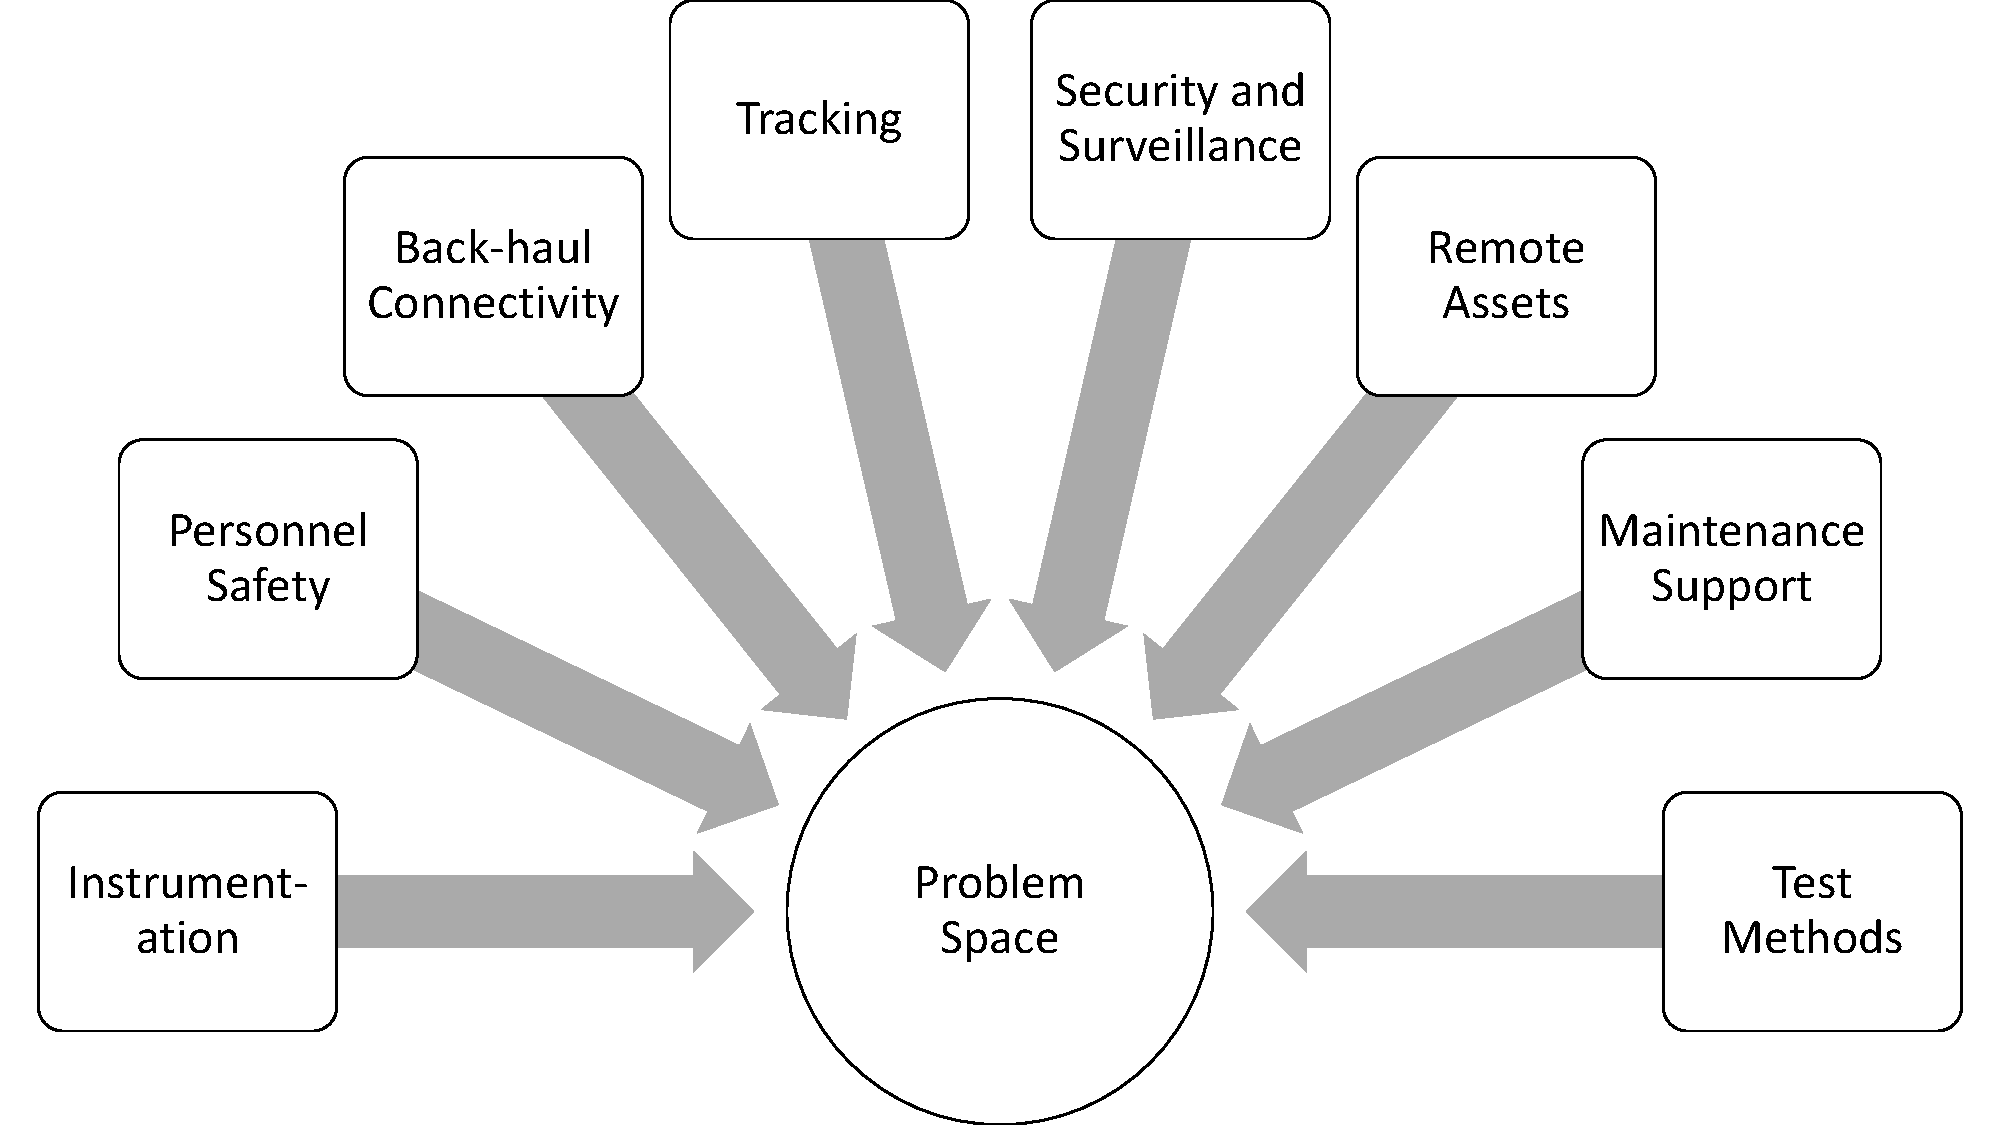
\includegraphics[width=\columnwidth]{images/probsp}
			\caption{Industrial wireless technologies are applicable across most aspects of an industrial operation.}
			\label{fig:problemspace}
		\end{figure}   
	
		% Table generated by Excel2LaTeX from sheet 'mapping'
		\begin{table*}[htbp]
			\setlength{\tabcolsep}{1.4pt}
			\centering
			\caption{Asserted applicability of wireless technologies.}
			\label{tbl:techmap}%
			\begin{adjustbox}{width=\textwidth}
				% Table generated by Excel2LaTeX from sheet 'mapping'
\begin{tabular}{l|l|ccccc|cccccc|cccc|cccc|ccccc|cccccc|ccc|ccc}
\multicolumn{1}{r}{} &
  \multicolumn{1}{r}{} &
  \begin{sideways}Process Monitoring\end{sideways} &
  \begin{sideways}Supervisory Control\end{sideways} &
  \begin{sideways}Feedback Control\end{sideways} &
  \begin{sideways}Alarm Conditions\end{sideways} &
  \multicolumn{1}{c}{\begin{sideways}In-situ Inspection\end{sideways}} &
  \begin{sideways}Factory Monitoring\end{sideways} &
  \begin{sideways}Assembly: Sensing\end{sideways} &
  \begin{sideways}Assembly: Actuation\end{sideways} &
  \begin{sideways}Robots: Supervision\end{sideways} &
  \begin{sideways}Robots: Feedback Control\end{sideways} &
  \multicolumn{1}{c}{\begin{sideways}Quality Inspection\end{sideways}} &
  \begin{sideways}Fall Prevention\end{sideways} &
  \begin{sideways}Confined Spaces\end{sideways} &
  \begin{sideways}Critical Event Detection\end{sideways} &
  \multicolumn{1}{c}{\begin{sideways}Human-Machine Colocation\end{sideways}} &
  \begin{sideways}Nearby or Indoor\end{sideways} &
  \begin{sideways}Distant: LOS\end{sideways} &
  \begin{sideways}Distant: BLOS\end{sideways} &
  \multicolumn{1}{c}{\begin{sideways}Geographically Remote\end{sideways}} &
  \begin{sideways}Indoor Machine Localization\end{sideways} &
  \begin{sideways}Materials in Storage\end{sideways} &
  \begin{sideways}Materials in Production\end{sideways} &
  \begin{sideways}Tools\end{sideways} &
  \multicolumn{1}{c}{\begin{sideways}Personnel\end{sideways}} &
  \begin{sideways}Voice and Video Communication\end{sideways} &
  \begin{sideways}Video Survellience\end{sideways} &
  \begin{sideways}Drone-based Surveillance\end{sideways} &
  \begin{sideways}Grounds Control\end{sideways} &
  \begin{sideways}Spectrum Monitoring Data\end{sideways} &
  \multicolumn{1}{c}{\begin{sideways}Personnel Authorization\end{sideways}} &
  \begin{sideways}Well-head Monitoring\end{sideways} &
  \begin{sideways}Pipeline Monitoring\end{sideways} &
  \multicolumn{1}{c}{\begin{sideways}Tank Level Monitoring\end{sideways}} &
  \begin{sideways}Machine Health Monitoring\end{sideways} &
  \begin{sideways}Building Automation\end{sideways} &
  \begin{sideways}Augmented Reality\end{sideways}
  \\
\multicolumn{1}{r}{} &
  \multicolumn{1}{r}{} &
  \multicolumn{5}{c|}{Flow-based} &
  \multicolumn{6}{c|}{Job-based} &
  \multicolumn{4}{c|}{Safety} &
  \multicolumn{4}{c|}{Back-haul} &
  \multicolumn{5}{c|}{Tracking} &
  \multicolumn{6}{c|}{Security} &
  \multicolumn{3}{c|}{Remote} &
  \multicolumn{3}{c}{Maint.}
  \\
\midrule
\multirow{2}[2]{*}{Home/Office} &
  IEEE 802.11 &
  \CIRCLE &
  \CIRCLE &
  \LEFTcircle &
  \LEFTcircle &
  - &
  \CIRCLE &
  \LEFTcircle &
  \LEFTcircle &
  \LEFTcircle &
  \LEFTcircle &
  \LEFTcircle &
  \fullmoon &
  \fullmoon &
  \LEFTcircle &
  \fullmoon &
  \CIRCLE &
  \CIRCLE &
  \CIRCLE &
  - &
  \LEFTcircle &
  \lightning &
  \lightning &
  \lightning &
  \multicolumn{1}{c}{\lightning} &
  \CIRCLE &
  \CIRCLE &
  \CIRCLE &
  \CIRCLE &
  \CIRCLE &
  \CIRCLE &
  \LEFTcircle &
  \fullmoon &
  \LEFTcircle &
  \LEFTcircle &
  \CIRCLE &
  \CIRCLE
  \\
 &
  IEEE 802.15.1 &
  \fullmoon &
  \fullmoon &
  \fullmoon &
  \fullmoon &
  \fullmoon &
  \fullmoon &
  \LEFTcircle &
  \LEFTcircle &
  \LEFTcircle &
  \fullmoon &
  \CIRCLE &
  \fullmoon &
  \LEFTcircle &
  \fullmoon &
  \fullmoon &
  \fullmoon &
  \fullmoon &
  \fullmoon &
  \fullmoon &
  \fullmoon &
  \fullmoon &
  \lightning &
  \CIRCLE &
  \LEFTcircle &
  \DOWNarrow &
  \DOWNarrow &
  \DOWNarrow &
  \fullmoon &
  \fullmoon &
  \LEFTcircle &
  \fullmoon &
  \fullmoon &
  \fullmoon &
  \LEFTcircle &
  \fullmoon &
  \DOWNarrow
  \\
\midrule
\multirow{4}[2]{*}{Industrial} &
  IEEE 802.15.4 TDMA &
  \CIRCLE &
  \CIRCLE &
  \LEFTcircle &
  \LEFTcircle &
  - &
  \CIRCLE &
  \clock &
  \clock &
  \clock &
  \clock &
  \LEFTcircle &
  \clock &
  \LEFTcircle &
  \LEFTcircle &
  \fullmoon &
  \DOWNarrow &
  \DOWNarrow &
  \DOWNarrow &
  \DOWNarrow &
  \LEFTcircle &
  \lightning &
  \lightning &
  \lightning &
  \LEFTcircle &
  \DOWNarrow &
  \DOWNarrow &
  \DOWNarrow &
  \LEFTcircle &
  \DOWNarrow &
  \fullmoon &
  \CIRCLE &
  \CIRCLE &
  \CIRCLE &
  \CIRCLE &
  \CIRCLE &
  \DOWNarrow
  \\
 &
  IEEE 802.15.4 CSMA &
  \LEFTcircle &
  \LEFTcircle &
  \fullmoon &
  \fullmoon &
  - &
  \CIRCLE &
  \clock &
  \clock &
  \clock &
  \clock &
  \LEFTcircle &
  \clock &
  \LEFTcircle &
  \LEFTcircle &
  \fullmoon &
  \DOWNarrow &
  \DOWNarrow &
  \DOWNarrow &
  \DOWNarrow &
  \LEFTcircle &
  \lightning &
  \lightning &
  \lightning &
  \LEFTcircle &
  \DOWNarrow &
  \DOWNarrow &
  \DOWNarrow &
  \LEFTcircle &
  \fullmoon &
  \fullmoon &
  \LEFTcircle &
  \LEFTcircle &
  \LEFTcircle &
  \CIRCLE &
  \CIRCLE &
  \DOWNarrow
  \\
 &
  IEEE 802.11 TDMA &
  \hexstar &
  \hexstar &
  \hexstar &
  \hexstar &
  - &
  \hexstar &
  \hexstar &
  \hexstar &
  \hexstar &
  \hexstar &
  \hexstar &
  \hexstar &
  \hexstar &
  \hexstar &
  \hexstar &
  - &
  - &
  - &
  - &
  \hexstar &
  - &
  - &
  - &
  - &
  - &
  - &
  - &
  \hexstar &
  - &
  - &
  \hexstar &
  \hexstar &
  \hexstar &
  \hexstar &
  \hexstar &
  -
  \\
 &
  VLBR WAN &
  \CIRCLE &
  \CIRCLE &
  \fullmoon &
  \LEFTcircle &
  - &
  \CIRCLE &
  \clock &
  \clock &
  \clock &
  \clock &
  \clock &
  \clock &
  \fullmoon &
  \fullmoon &
  \fullmoon &
  \DOWNarrow &
  \DOWNarrow &
  \DOWNarrow &
  \DOWNarrow &
  \LEFTcircle &
  \LEFTcircle &
  \LEFTcircle &
  \LEFTcircle &
  \LEFTcircle &
  \DOWNarrow &
  \DOWNarrow &
  \DOWNarrow &
  \clock &
  \fullmoon &
  \fullmoon &
  \fullmoon &
  \fullmoon &
  \fullmoon &
  \LEFTcircle &
  \LEFTcircle &
  \fullmoon
  \\
\midrule
\multirow{3}[2]{*}{Satellite} &
  Geostationary &
  \LEFTcircle &
  \LEFTcircle &
  \fullmoon &
  \fullmoon &
  \fullmoon &
  \fullmoon &
  \fullmoon &
  \fullmoon &
  \fullmoon &
  \fullmoon &
  \fullmoon &
  \fullmoon &
  \fullmoon &
  \fullmoon &
  \fullmoon &
  \fullmoon &
  \fullmoon &
  \fullmoon &
  \LEFTcircle &
  \fullmoon &
  \fullmoon &
  \fullmoon &
  \fullmoon &
  \fullmoon &
  \LEFTcircle &
  \LEFTcircle &
  \fullmoon &
  \LEFTcircle &
  \LEFTcircle &
  \LEFTcircle &
  \LEFTcircle &
  \LEFTcircle &
  \LEFTcircle &
  \fullmoon &
  \fullmoon &
  \LEFTcircle
  \\
 &
  Low-earth Orbit &
  \LEFTcircle &
  \LEFTcircle &
  \fullmoon &
  \fullmoon &
  \fullmoon &
  \fullmoon &
  \fullmoon &
  \fullmoon &
  \fullmoon &
  \fullmoon &
  \fullmoon &
  \fullmoon &
  \fullmoon &
  \fullmoon &
  \fullmoon &
  \fullmoon &
  \fullmoon &
  \LEFTcircle &
  \LEFTcircle &
  \fullmoon &
  \fullmoon &
  \fullmoon &
  \fullmoon &
  \fullmoon &
  \LEFTcircle &
  \LEFTcircle &
  \LEFTcircle &
  \LEFTcircle &
  \LEFTcircle &
  \LEFTcircle &
  \LEFTcircle &
  \LEFTcircle &
  \LEFTcircle &
  \LEFTcircle &
  \fullmoon &
  \LEFTcircle
  \\
 &
  VLBR WAN &
  \LEFTcircle &
  \LEFTcircle &
  \fullmoon &
  \LEFTcircle &
  \fullmoon &
  \clock &
  \clock &
  \clock &
  \clock &
  \clock &
  \clock &
  \clock &
  \fullmoon &
  \fullmoon &
  \fullmoon &
  \DOWNarrow &
  \DOWNarrow &
  \DOWNarrow &
  \DOWNarrow &
  \fullmoon &
  \fullmoon &
  \fullmoon &
  \fullmoon &
  \LEFTcircle &
  \DOWNarrow &
  \DOWNarrow &
  \DOWNarrow &
  \LEFTcircle &
  \fullmoon &
  \fullmoon &
  \fullmoon &
  \fullmoon &
  \fullmoon &
  \LEFTcircle &
  \fullmoon &
  \DOWNarrow
  \\
\midrule
Tracking &
  RFID &
  - &
  - &
  - &
  - &
  - &
  - &
  - &
  - &
  - &
  - &
  - &
  - &
  - &
  - &
  - &
  - &
  - &
  - &
  - &
  \fullmoon &
  \CIRCLE &
  \CIRCLE &
  \CIRCLE &
  \CIRCLE &
  - &
  - &
  - &
  - &
  - &
  - &
  - &
  - &
  - &
  - &
  - &
  -
  \\
\midrule
\multirow{2}[1]{*}{Optical} &
  Indoor Dispersive &
  \hexstar &
  \hexstar &
  \hexstar &
  \hexstar &
  \fullmoon &
  \hexstar &
  \hexstar &
  \hexstar &
  \hexstar &
  \hexstar &
  \hexstar &
  \hexstar &
  \hexstar &
  \hexstar &
  \hexstar &
  \hexstar &
  \fullmoon &
  \fullmoon &
  \fullmoon &
  \hexstar &
  \lightning &
  \lightning &
  \lightning &
  \lightning &
  \hexstar &
  \hexstar &
  \fullmoon &
  \fullmoon &
  \hexstar &
  \fullmoon &
  \fullmoon &
  \fullmoon &
  \fullmoon &
  \hexstar &
  \fullmoon &
  \fullmoon
  \\
 &
  Free-space &
  \LEFTcircle &
  \LEFTcircle &
  \LEFTcircle &
  \LEFTcircle &
  \fullmoon &
  \fullmoon &
  \fullmoon &
  \fullmoon &
  \fullmoon &
  \fullmoon &
  \fullmoon &
  \fullmoon &
  \fullmoon &
  \fullmoon &
  \fullmoon &
  \CIRCLE &
  \CIRCLE &
  \CIRCLE &
  \fullmoon &
  \LEFTcircle &
  \fullmoon &
  \fullmoon &
  \fullmoon &
  \fullmoon &
  \CIRCLE &
  \CIRCLE &
  \fullmoon &
  \fullmoon &
  \fullmoon &
  \fullmoon &
  \CIRCLE &
  \fullmoon &
  \CIRCLE &
  \fullmoon &
  \fullmoon &
  \CIRCLE
  \\
\midrule
\multirow{3}[2]{*}{Cellular} &
  Legacy &
  \LEFTcircle &
  \LEFTcircle &
  \fullmoon &
  \fullmoon &
  - &
  \fullmoon &
  \fullmoon &
  \fullmoon &
  \fullmoon &
  \fullmoon &
  \fullmoon &
  \clock &
  \clock &
  \clock &
  \clock &
  \LEFTcircle &
  \LEFTcircle &
  \LEFTcircle &
  \LEFTcircle &
  \fullmoon &
  \fullmoon &
  \fullmoon &
  \fullmoon &
  \fullmoon &
  \fullmoon &
  \fullmoon &
  \fullmoon &
  \fullmoon &
  \hexstar &
  \LEFTcircle &
  \LEFTcircle &
  \LEFTcircle &
  \LEFTcircle &
  \LEFTcircle &
  \DOWNarrow &
  \DOWNarrow
  \\
 &
  4G &
  \LEFTcircle &
  \LEFTcircle &
  \fullmoon &
  \clock &
  - &
  \fullmoon &
  \fullmoon &
  \fullmoon &
  \fullmoon &
  \fullmoon &
  \fullmoon &
  \clock &
  \clock &
  \clock &
  \clock &
  \LEFTcircle &
  \LEFTcircle &
  \LEFTcircle &
  \LEFTcircle &
  \fullmoon &
  \fullmoon &
  \fullmoon &
  \fullmoon &
  \fullmoon &
  \CIRCLE &
  \CIRCLE &
  \LEFTcircle &
  \CIRCLE &
  \CIRCLE &
  \CIRCLE &
  \LEFTcircle &
  \LEFTcircle &
  \LEFTcircle &
  \fullmoon &
  \fullmoon &
  \fullmoon
  \\
 &
  5G &
  \hexstar &
  \hexstar &
  \hexstar &
  \hexstar &
  - &
  \hexstar &
  \hexstar &
  \hexstar &
  \hexstar &
  \hexstar &
  \hexstar &
  \hexstar &
  \hexstar &
  \hexstar &
  \hexstar &
  \CIRCLE &
  \CIRCLE &
  \CIRCLE &
  \fullmoon &
  \hexstar &
  \hexstar &
  \hexstar &
  \hexstar &
  \hexstar &
  \hexstar &
  \hexstar &
  \hexstar &
  \hexstar &
  \hexstar &
  \hexstar &
  \hexstar &
  \hexstar &
  \hexstar &
  \hexstar &
  \hexstar &
  \hexstar
  \\
\midrule
\multicolumn{1}{l|}{Land-mobile} &
  All types &
  \fullmoon &
  \fullmoon &
  \fullmoon &
  \fullmoon &
  \fullmoon &
  \fullmoon &
  \fullmoon &
  \fullmoon &
  \fullmoon &
  \fullmoon &
  \fullmoon &
  \fullmoon &
  \fullmoon &
  \fullmoon &
  \fullmoon &
  \DOWNarrow &
  \DOWNarrow &
  \fullmoon &
  \fullmoon &
  \fullmoon &
  \fullmoon &
  \fullmoon &
  \fullmoon &
  \fullmoon &
  \LEFTcircle &
  \fullmoon &
  \fullmoon &
  \CIRCLE &
  \fullmoon &
  \LEFTcircle &
  \fullmoon &
  \fullmoon &
  \fullmoon &
  \fullmoon &
  \fullmoon &
  \multicolumn{1}{c}{\fullmoon}
  \\
\midrule
Specialty &
  Leaky Coax &
  \LEFTcircle &
  \LEFTcircle &
  - &
  \LEFTcircle &
  \LEFTcircle &
  \LEFTcircle &
  - &
  - &
  \fullmoon &
  \fullmoon &
  - &
  \fullmoon &
  \LEFTcircle &
  \LEFTcircle &
  - &
  \LEFTcircle &
  \fullmoon &
  \fullmoon &
  \fullmoon &
  \LEFTcircle &
  \CIRCLE &
  \CIRCLE &
  \fullmoon &
  \fullmoon &
  \fullmoon &
  \fullmoon &
  \fullmoon &
  \CIRCLE &
  \fullmoon &
  \CIRCLE &
  \fullmoon &
  \fullmoon &
  \fullmoon &
  \LEFTcircle &
  \LEFTcircle &
  \fullmoon
  \\
\bottomrule
\end{tabular}%

			\end{adjustbox}
			\vspace{3pt}
			\raggedright
			
			Legend: 
			\CIRCLE:~{Technology fully supports problem domain,}
			\LEFTcircle:~{Supports problem domain with practicality, throughput, latency, reliability, or energy limitations,}
			\lightning:~{Energy requirements of assumed battery-powered devices prevent applicability,}
			\clock:~{Latency prevent applicability,}
			\DOWNarrow:~{Throughput prevents applicability,}
			\hexstar:~{Emerging technology or evolution may support problem domain,}
			\fullmoon:~{Not recommended,}
			-:~{Not considered by authors.}
			% \newline
			% \noindent\makebox[\linewidth]{\rule{\linewidth}{0.4pt}}
			% This table represents assertions by the authors of applicability of wireless technologies to industrial control systems problem domains based on industry practice and intent of the technology.  The authors assert that the problem domains and wireless technologies included within this table represent the majority  of problems found within industry and the existing technologies that may be applied.  In some cases, modifications may be made to the listed technologies resulting in applicability to a specified problem.  Very low bit rate (VLBR) wide area networks (WAN) are assumed to have an infrastructure topology. 
			% \noindent\makebox[\linewidth]{\rule{\linewidth}{0.4pt}}
		\end{table*}%
	
		%
		% SYSML FIGURES
		%
		\begin{figure}[!tbhp]
			\centering
			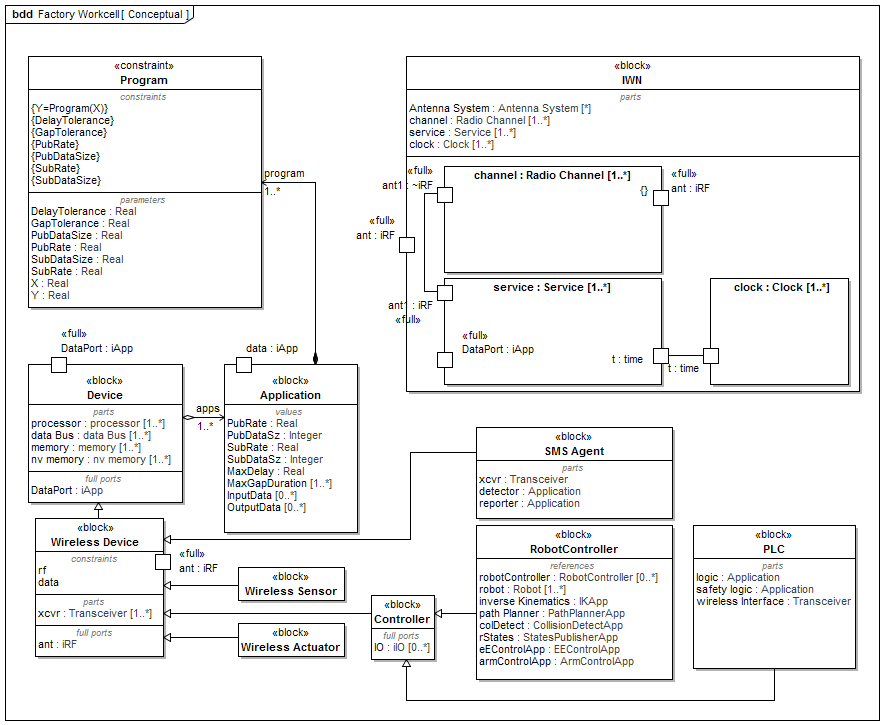
\includegraphics[width=0.95\textwidth]{images/bdd__Factory_Workcell__Conceptual}
			\caption{SysML conceptual model of the factory workcell.}
			\label{fig:sysmlex}
		\end{figure}
	
		%
		% GDB FIGURES
		%
		\begin{figure*}
			\centering
			%	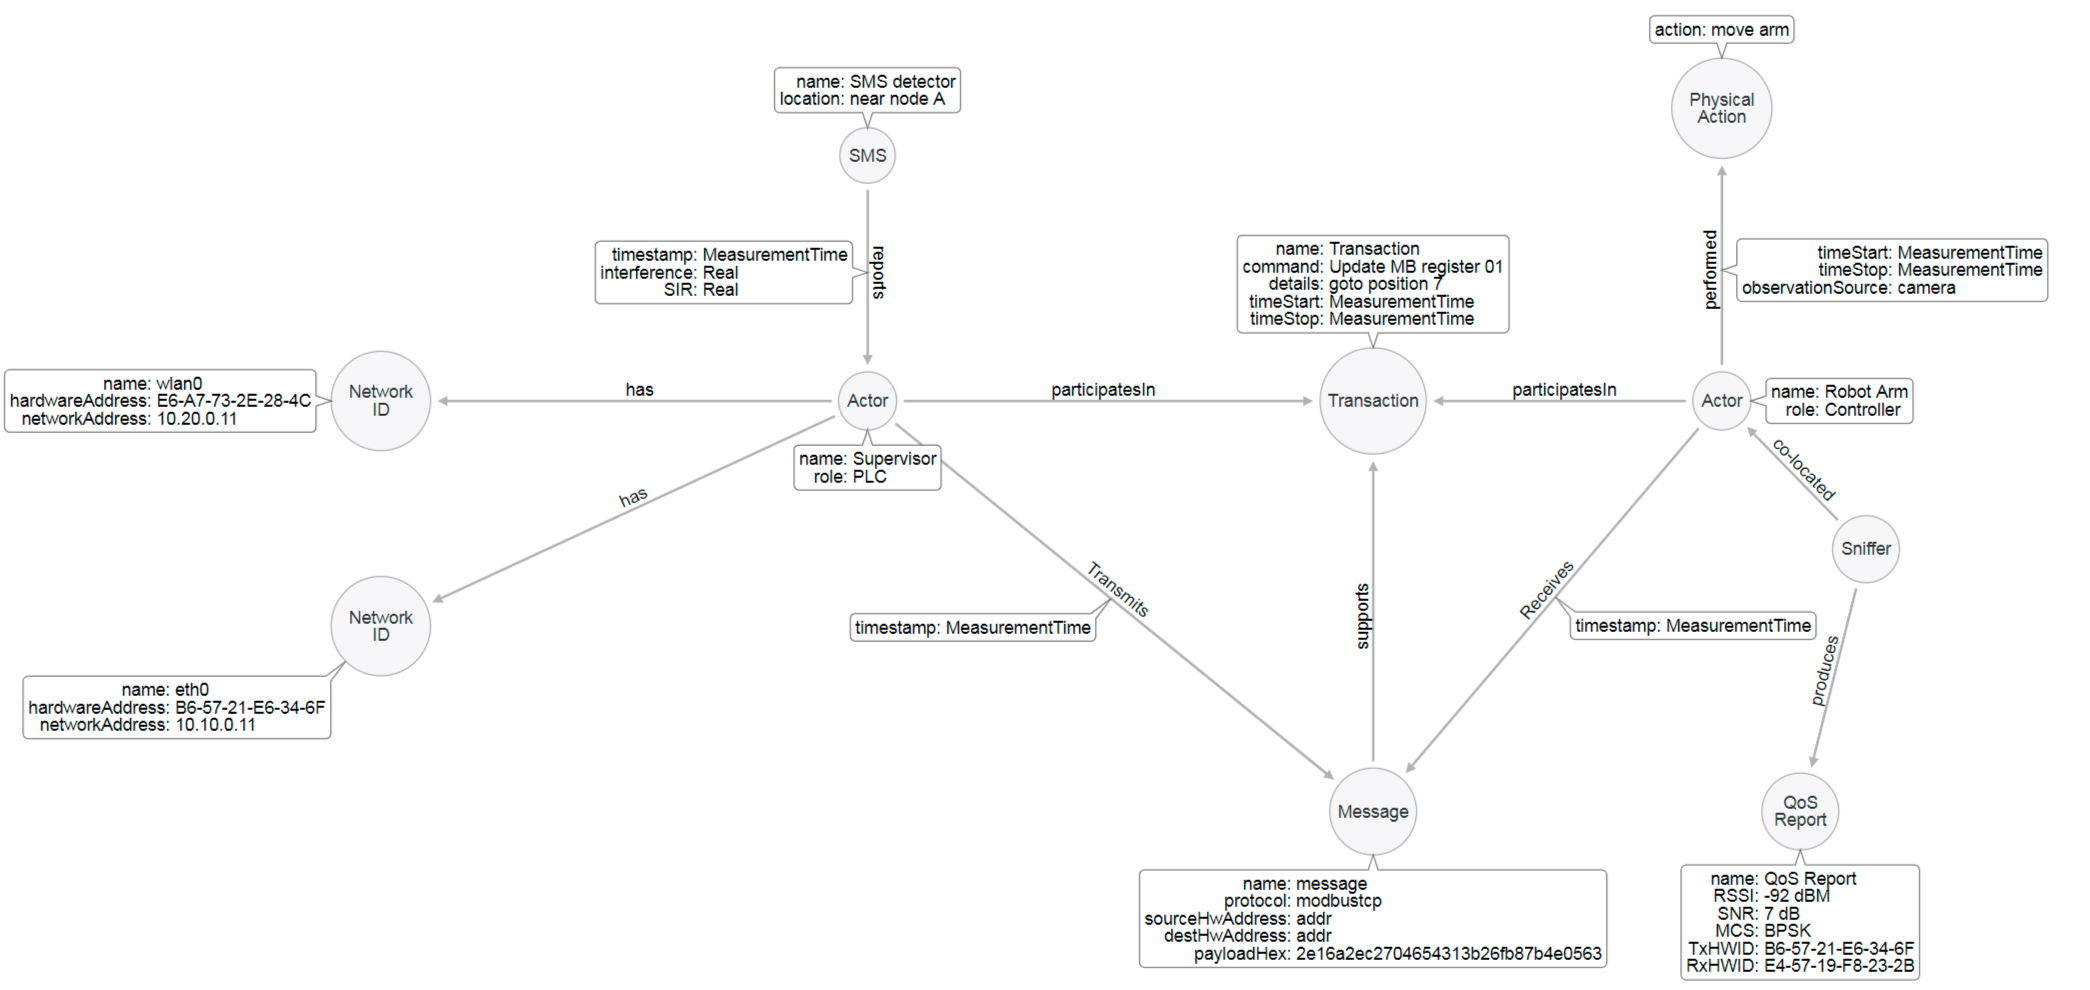
\includegraphics[width=\textwidth,trim=50 50 50 50, clip]{figures/database/arrows-schema.PNG}
			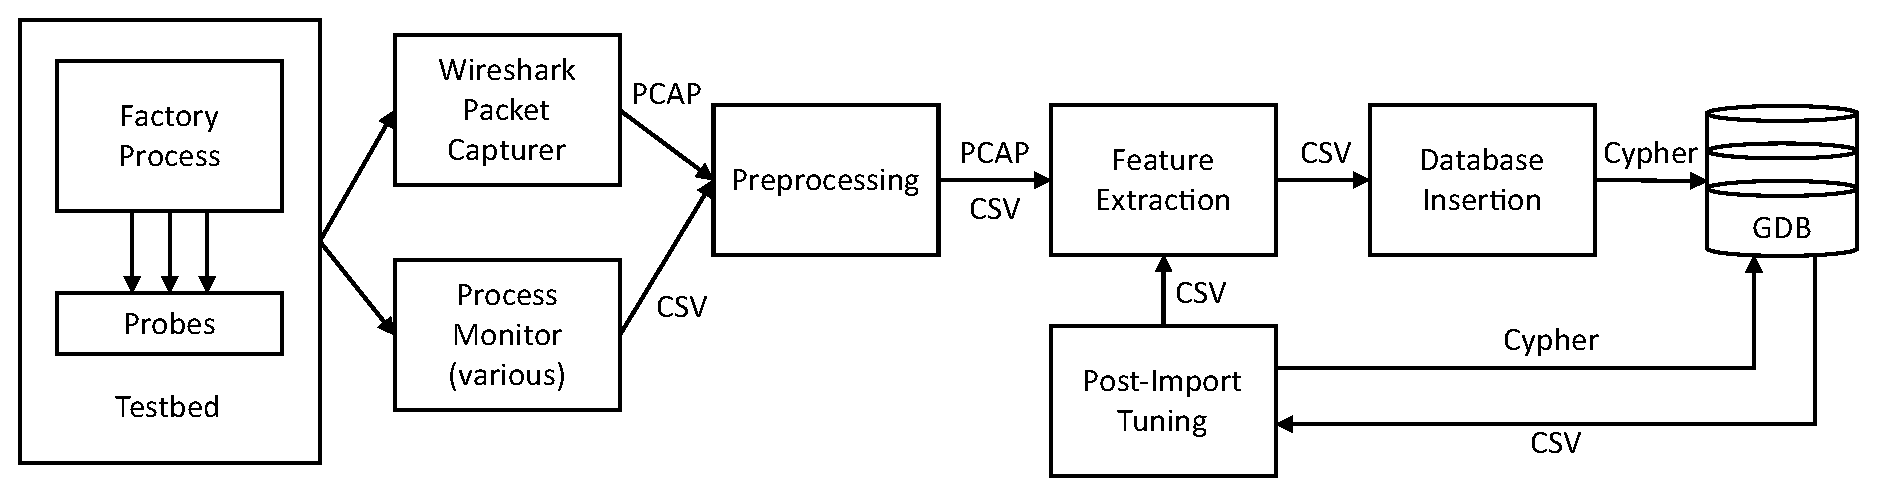
\includegraphics[width=\linewidth]{images/info_workflow_tii.eps}
			\caption{Data processing flow from factory work-cell to database}
			\label{gdbappl:fig:database:work-flow}
		\end{figure*}
	
		\begin{figure*}
			\centering
			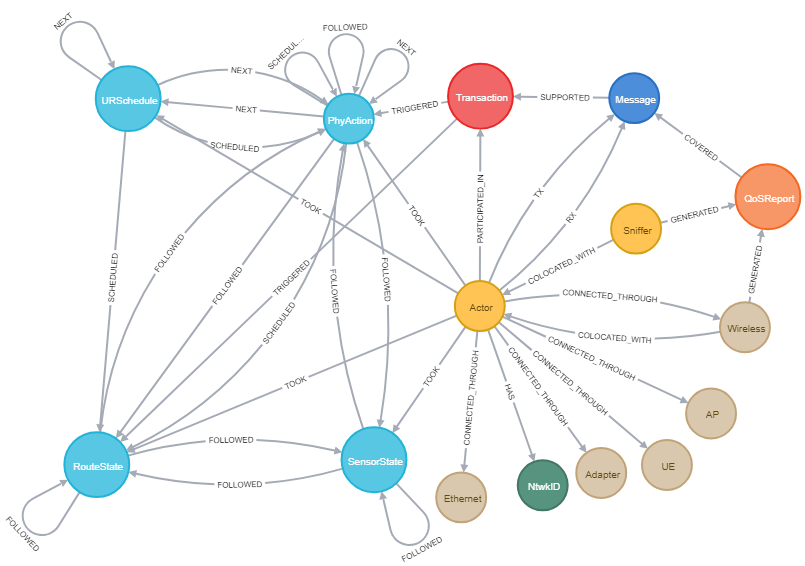
\includegraphics[width=\linewidth]{images/graph_schema_updated_2.png}
			\caption{Realized schema of the graph database fully populated after capturing network and operational data from the NIST industrial wireless testbed. \vspace{-0.2in}}
			\label{gdbappl:fig:real-schema}
		\end{figure*}
	
	
		%
		% MACHINE LEARNING FIGURES
		%
		\begin{figure}[!tbp]
			\centering
			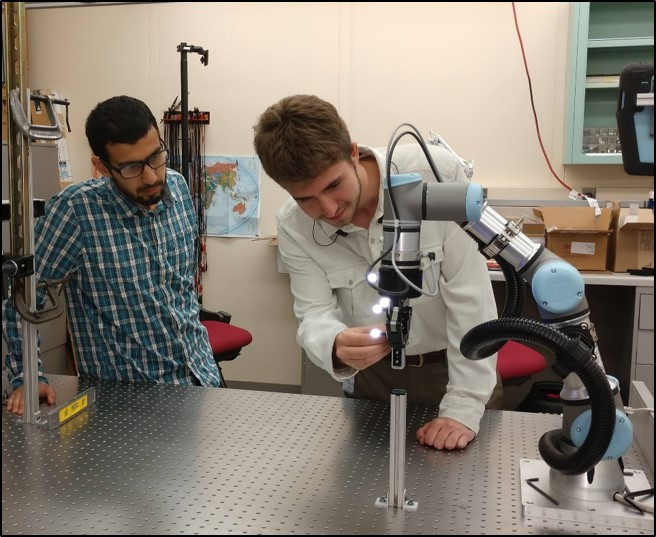
\includegraphics[width=0.65\columnwidth]{images/PlungerExperiment}
			\caption{A photograph of the robot force-seeking apparatus used for the machine learning experiment.  The photo shows the robotic arm, the spring-based plunger, and the visual markers used for position tracking.}
			\label{fig:photo-forceseeker}
		\end{figure}
		
		\begin{figure}[!ht]
			\begin{subfigure}{.5\linewidth}
				\centering
				% include first image
				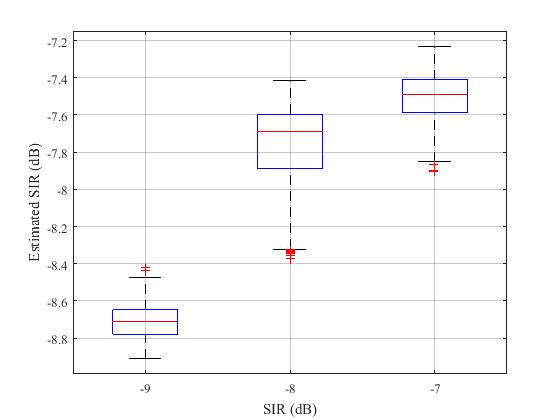
\includegraphics[width=.99\linewidth]{images/BP_1}  
				\caption{[$M=100$}
				\label{ftml-conf:fig:results-BP-1}
			\end{subfigure}
			\begin{subfigure}{.5\linewidth}
				\centering
				% include second image
				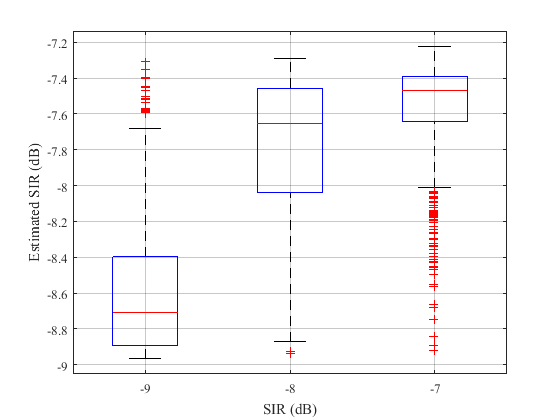
\includegraphics[width=.99\linewidth]{images/BP_2}  
				\caption{[$M=1$}
				\label{ftml-conf:fig:results-BP-2}
			\end{subfigure}
			\caption{Predicted SIR versus actual SIR for the cases of~\protect\subref{ftml-conf:fig:results-BP-1} $M=100$ and~\protect\subref{ftml-conf:fig:results-BP-2} $M=1$. The box plots show the median value while the bottom and top edges of the box indicate the 25th and 75th percentiles.  Statistical outliers are shown as red $+$ signs.}
			\label{ftml-conf:fig:results-BP}
		\end{figure}
	
	
\end{document}
